\documentclass[notes,serif]{beamer}
\usepackage{graphicx}
\usepackage{url}
\usepackage{clrscode}

% You should run 'pdflatex' TWICE, because of TOC issues.

\mode<presentation>
{
  % A tip: pick a theme you like first, and THEN modify the color theme, and then add math content.
  % Warsaw is the theme selected by default in Beamer's installation sample files.

  %%%%%%%%%%%%%%%%%%%%%%%%%%%% THEME
  %\usetheme{AnnArbor}
  %\usetheme{Antibes}
  %\usetheme{Bergen}
  %\usetheme{Berkeley}
  %\usetheme{Berlin}
  %\usetheme{Boadilla}
  %\usetheme{boxes}
  %\usetheme{CambridgeUS}
  %\usetheme{Copenhagen}
  %\usetheme{Darmstadt}
  %\usetheme{default}
  %\usetheme{Dresden}
  %\usetheme{Frankfurt}
  %\usetheme{Goettingen}
  %\usetheme{Hannover}
  %\usetheme{Ilmenau}
  %\usetheme{JuanLesPins}
  %\usetheme{Luebeck}
  %\usetheme{Madrid}
  %\usetheme{Malmoe}
  %\usetheme{Marburg}
  %\usetheme{Montpellier}
  %\usetheme{PaloAlto}
  %\usetheme{Pittsburgh}
  %\usetheme{Rochester}
  %\usetheme{Singapore}
  %\usetheme{Szeged}
  \usetheme{Warsaw}

  %%%%%%%%%%%%%%%%%%%%%%%%%%%% COLOR THEME
  %\usecolortheme{albatross}
  %\usecolortheme{beetle}
  %\usecolortheme{crane}
  \usecolortheme{default}
  %\usecolortheme{dolphin}
  %\usecolortheme{dove}
  %\usecolortheme{fly}
  %\usecolortheme{lily}
  %\usecolortheme{orchid}
  %\usecolortheme{rose}
  %\usecolortheme{seagull}
  %\usecolortheme{seahorse}
  %\usecolortheme{sidebartab}
  %\usecolortheme{structure}
  %\usecolortheme{whale}

  %%%%%%%%%%%%%%%%%%%%%%%%%%%% OUTER THEME
  %\useoutertheme{default}
  %\useoutertheme{infolines}
  %\useoutertheme{miniframes}
  %\useoutertheme{shadow}
  %\useoutertheme{sidebar}
  %\useoutertheme{smoothbars}
  %\useoutertheme{smoothtree}
  %\useoutertheme{split}
  %\useoutertheme{tree}

  %%%%%%%%%%%%%%%%%%%%%%%%%%%% INNER THEME
  %\useinnertheme{circles}
  %\useinnertheme{default}
  %\useinnertheme{inmargin}
  %\useinnertheme{rectangles}
  %\useinnertheme{rounded}

  %%%%%%%%%%%%%%%%%%%%%%%%%%%%%%%%%%%

  \setbeamercovered{transparent} % or whatever (possibly just delete it)
  % To change behavior of \uncover from graying out to totally invisible, can change \setbeamercovered to invisible instead of transparent. apparently there are also 'dynamic' modes that make the amount of graying depend on how long it'll take until the thing is uncovered.

}


% Get rid of nav bar
\beamertemplatenavigationsymbolsempty

% Use short top
%\usepackage[headheight=12pt,footheight=12pt]{beamerthemeboxes}
%\addheadboxtemplate{\color{black}}{
%\hskip0.3cm
%\color{white}
%\insertshortauthor \ \ \ \
%\insertframenumber \ \ \ \ \ \ \
%\insertsection \ \ \ \ \ \ \ \ \ \ \ \ \ \ \ \ \  \insertsubsection
%\hskip0.3cm}
%\addheadboxtemplate{\color{black}}{
%\color{white}
%\ \ \ \
%\insertsection
%}
%\addheadboxtemplate{\color{black}}{
%\color{white}
%\ \ \ \
%\insertsubsection
%}

% Insert frame number at bottom of the page.
\usefoottemplate{\hfil\tiny{\color{black!90}\insertframenumber}}

\usepackage[english]{babel}
\usepackage[latin1]{inputenc}

\usepackage{times}
\usepackage[T1]{fontenc}

\title{The Design and Analysis of Algorithms}
\subtitle{Lecture 1}

\author{Lei Wang}

\institute{Dalian University of Technology}

%\date{Date}

\subject{Talks}

\def\defn#1{{\color{red} #1}}

\begin{document}

\begin{frame}
  \titlepage
\end{frame}

\begin{frame}
  \frametitle{Get Started}
  \tableofcontents
\end{frame}

\section{Course Info}

\begin{frame}
\frametitle{Course Info}
\begin{itemize}
  \item Instructor: Lei Wang, lei.wang@dlut.edu.cn, tel: 6227 4394
  \item Textbook: {\bf Introduction to Algorithms}, by Thomas Cormen {\em et al.}, aka, CLRS.
  \item Courseware: MIT Open Coursework \\
  {\small \url{http://ocw.mit.edu/OcwWeb/Electrical-Engineering-and-Computer-Science/6-046JFall-2005/CourseHome/index.htm}}
  \item Call for volunteer TAs
  \item {\LaTeX} is strongly recommended
\end{itemize}
\end{frame}

\section{Overview}

\subsection{Goals}

\begin{frame}
\frametitle{Goals}

\begin{itemize}
    \item Start using frameworks for describing and analyzing algorithms.
    \item Examine two algorithms for sorting: insertion sort and merge sort.
    \item See how to describe algorithms in pseudocode.
    \item Begin using asymptotic notation to express running-time analysis.
    \item Learn the technique of ``divide and conquer'' in the context of merge sort.
\end{itemize}

%Preliminary things that we must cover before going on:
%
%\begin{columns}
%
%\column{0.5\textwidth}
%
%Working inside a column...
%
%\begin{block}{Blocks default to blue}
%\begin{itemize}
%\item Itemize
%\item Itemize
%\end{itemize}
%\end{block}
%
%\begin{alertblock}{Alert Blocks are red (by default)}
%\begin{enumerate}
%\item Enumerate
%\item Enumerate
%\end{enumerate}
%\end{alertblock}
%
%\column{0.5\textwidth}
%
%\hyperlink{post_equalities}{\beamergotobutton{Skip rest of $\mathbb{R}^{n+1}$}}
%
%This is a precursor to studying \defn{integrals}:
%\begin{equation*}
%\int_a^b f(x)\ dx
%\end{equation*}
%
%\begin{exampleblock}{Example blocks for green}
%\begin{equation}
%\sum_{i=1}^\infty \frac1{n^2} = \frac\pi6
%\end{equation}
%\end{exampleblock}
%
%\pause\uncover{
%  This is a pause/uncover...\footnote{Use them for ``animation'' effect.}
%}
%
%%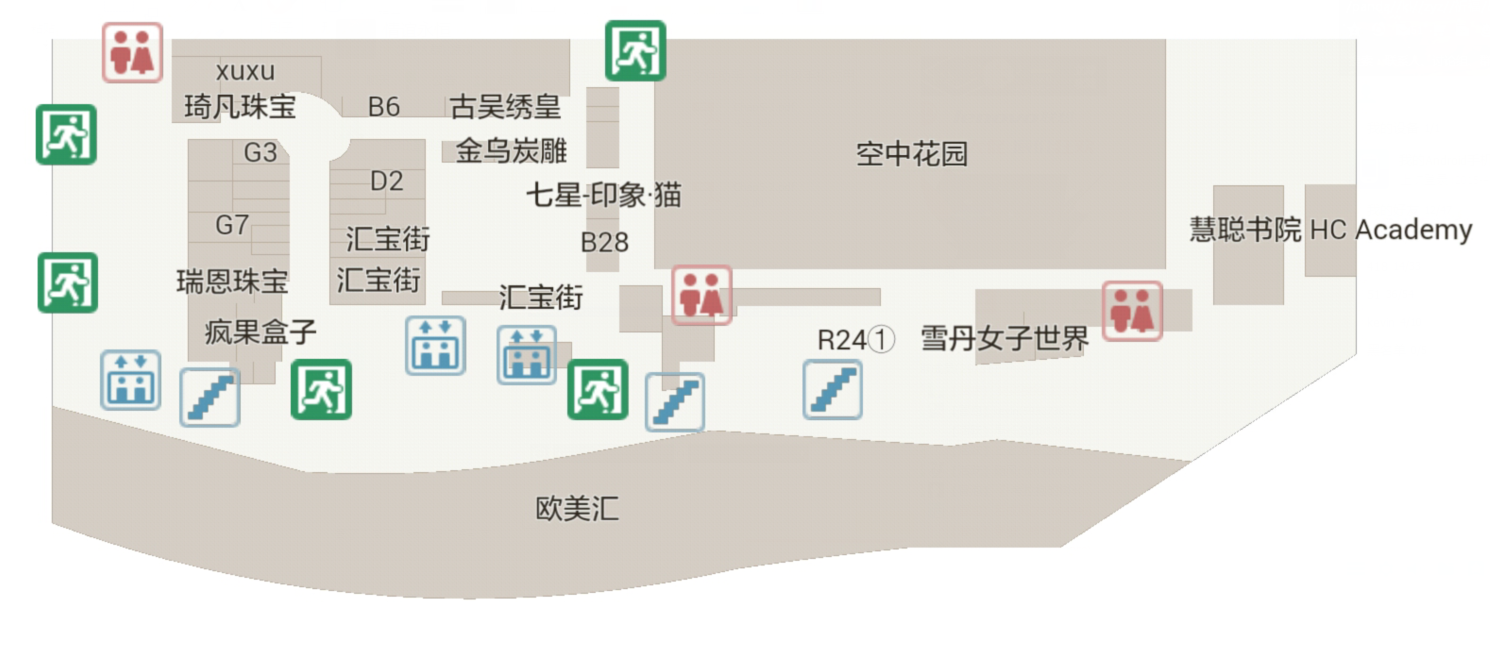
\includegraphics[width=2in]{example.jpg}
%
%\end{columns}
%
\end{frame}

%\subsection{Subsection 2}
%
%\begin{frame}
%\frametitle{Themes and TOC Space-Budgeting Issues}
%
%\hypertarget{post_equalities}{}
%
%A comment: I put all of these generically-named sections and subsections so that you can see what the different themes do to them.  If you happen to have a lot of sections and subsections (for example), then the Warsaw theme tends to take up a lot of space at the top.
%\begin{itemize}
%\item You can uncomment some code I have near the top that will just show the CURRENT section/subsection
%\item Or, if you don't like that, try using a theme that has the TOC run down a left-hand or right-hand column.  What you lose horizontally, you gain vertically.
%\end{itemize}
%
%\end{frame}
%
%\subsection{Subsection 3}
%
%\begin{frame}
%\frametitle{On Frame Titles}
%
%Good form apparently dictates that frames are supposed to have a title.  Titles should be informative.  ``Proof of Riemann Hypothesis'' beats ``Proof'' as a frame title (just in case an audience member zoned out at some point).
%
%\end{frame}

\section{Insertion Sort}

\subsection{Insertion sort}

\begin{frame}
  \frametitle{The sorting problem}
  \begin{block}{}
    {\bf Input:} A sequence of $n$ numbers $\langle a_1, a_2, \dots, a_n \rangle$.
  \end{block}
  \begin{block}{}
    {\bf Output:} A permutation (reordering) $\langle a_1', a_2', \dots, a_n' \rangle$ of the input sequence such that $a_1' \le a_2' \le \cdots \le a_n'$.
  \end{block}
  \begin{alertblock}{\bf Solution}
    {\bf Algorithm:} a well-defined computational procedure that takes some value, or set of values, as input and produces some value, or set of values, as output.
  \end{alertblock}
\end{frame}

\begin{frame}
  \frametitle{Insertion sort}
  \begin{itemize}
    \item A good algorithm for sorting a {\color{red}small} number of elements.
    \item It works the way you might sort a hand of playing cards.
  \end{itemize}
  \begin{block}{}
      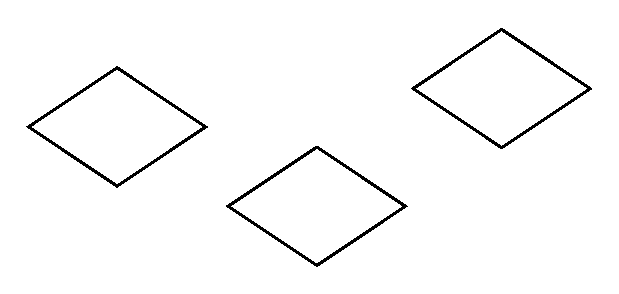
\includegraphics[height=4.5cm]{insertion_sort_a}
  \end{block}
\end{frame}

\subsection{Correctness}
\begin{frame}
  \frametitle{Correctness}
  We often use a {\bf \em loop invariant} to show the correctness of an algorithm.
  \begin{exampleblock}{Loop invariant for I\textsc{nsertion-\textnormal{s}ort}}
    At the start of each iteration of the ``outer'' {\bf for} loop---the
loop indexed by j---the subarray $A[1 . . j-1]$ consists of the elements originally
in $A[1 . . j-1]$ but in {\bf sorted} order.
  \end{exampleblock}
  \begin{block}{Three parts to prove correctness}
  \begin{itemize}
    \item {\bf Initialization:} It is true prior to the first iteration of the loop.
    \item {\bf Maintenance:}  If it is true before an iteration of the loop, it remains true before the
next iteration.
    \item {\bf Termination:} When the loop terminates, the invariant---usually along with the
reason that the loop terminated---gives us a useful property that helps show that the algorithm is correct.
  \end{itemize}
  \end{block}
\end{frame}

\begin{frame}
\frametitle{Using loop invariants is like mathematical induction}
\begin{itemize}
  \item To prove that a property holds, you prove a base case and an inductive step.
  \item Showing that the invariant holds before the first iteration is like the base case.
  \item Showing that the invariant holds from iteration to iteration is like the inductive
step.
  \item The termination part differs from the usual use of mathematical induction, in
which the inductive step is used infinitely. We stop the ``induction'' when the
loop terminates.
  \item We can show the three parts in any order.
\end{itemize}
\end{frame}

\begin{frame}
\frametitle{Example for insertion sort}
  \begin{exampleblock}{The three parts for insertion sort}
  \begin{itemize}
    \item {\bf Initialization:} Just before the first iteration, $j = 2$. The subarray $A[1 . . j-1]$
is the single element $A[1]$, which is the element originally in $A[1]$, and it is trivially sorted.
    \item {\bf Maintenance:}  we note that the body of the inner while loop works by moving
$A[j-1]$, $A[ j-2]$, $A[ j-3]$, and so on, by one position to the right until the proper position for {\em key} (which has the value that started out in $A[ j ]$) is found.  At that point, the value of {\em key} is placed into this position.
    \item {\bf Termination:} The outer for loop ends when $j > n$; this occurs when $j = n + 1$.
Thus, $j - 1 = n$. Plugging $n$ in for $j - 1$ in the loop invariant, $A[1 . . n]$ consists of the elements originally in $A[1 . . n]$ but in sorted order. The entire array is sorted!
  \end{itemize}
  \end{exampleblock}
\end{frame}

\section{Analyzing Algorithms}

\subsection{RAM Model}

\begin{frame}
\frametitle{Random-access machine (RAM) model}
\begin{itemize}
  \item Instructions are executed one after another. No concurrent operations.
  \item It's too tedious to define each of the instructions and their associated time costs.
  \item Instead, we recognize that we'll use instructions commonly found in real computers.

    \begin{itemize}
      \item Arithmetic: add, subtract, multiply, divide, remainder, floor, ceiling; shift left/shift right (good for multiplying/dividing by $2^k$).
      \item Data movement: load, store, copy.
      \item Control: conditional/unconditional branch, subroutine call and return.
    \end{itemize}
    Each of these instructions takes a constant amount of time.
\end{itemize}
\end{frame}

\subsection{Running Time}
\begin{frame}
\frametitle{Running time}
On a particular input, {\bf \em the running time} is the number of primitive operations (steps) executed.
\begin{itemize}
  \item Want to define steps to be machine-independent.
  \item Each line of pseudocode requires a constant amount of time.
  \item One line may take a different amount of time than another, but each execution
of line $i$ takes the same amount of time $c_i$.
  \item This is assuming that the line consists only of primitive operations.
\end{itemize}
\begin{alertblock}{}
  The running time of an algorithm is:
  $$\sum_{\textnormal{all statements}}{\textnormal{(cost of statement)}} \times \textnormal {(\# of times statement is executed)}$$
\end{alertblock}
\end{frame}

\begin{frame}
\frametitle{Analysis of insertion sort}
\begin{exampleblock}{Pseudocode with cost line by line}
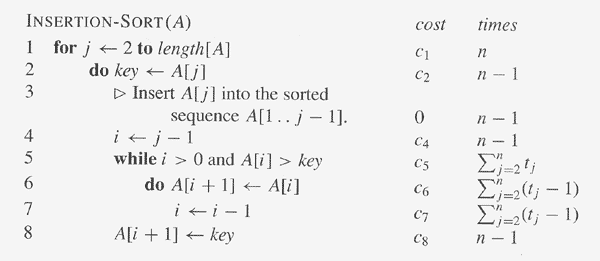
\includegraphics[height=3.6cm]{insertion_sort_a2}
\end{exampleblock}
\begin{block}{The running time of Insertion-Sort}
  $
  \begin{array}{lll}
    T(n) &=& c_1 n + c_2 (n-1) + c_4 (n-1) + c_5 \sum_{j=2}^n t_j \\
            & &  +\; c_6 \sum_{j=2}^n (t_j-1) + c_7 \sum_{j=2}^n (t_j-1) + c_8 (n-1)
  \end{array}
  $
\end{block}
\end{frame}

\begin{frame}
\frametitle{Analysis of insertion sort, (cont.)}
\begin{block}{\bf Best case:}
  \begin{eqnarray*}
  T(n) &=& c_1 n + c_2 (n-1) + c_4(n-1) + c_5(n-1) + c_8(n-1) \\
          &=& (c_1 + c_2 + c_4 + c_5 + c_8) n - (c_2 + c_4 + c_5 + c_8) \\
          &=& an + b.
  \end{eqnarray*}
\end{block}
\begin{block}{\bf Worst case:}
  \begin{eqnarray*}
  T(n) &=& c_1 n + c_2 (n-1) + c_4(n-1) + c_5({{n(n+1)} \over 2} -1) \\
          &  & + \; c_6({{n(n-1)} \over 2}) + c_7({{n(n-1)} \over 2}) + c_8(n-1) \\
%          &=& (c_1 + c_2 + c_4 + c_5 + c_8) n - (c_2 + c_4 + c_5 + c_8) \\
          &=& an^2 + bn + c.
  \end{eqnarray*}
\end{block}
\end{frame}

\begin{frame}
\frametitle{Worst-case and average-case analysis}
We usually concentrate on finding the {\bf \em worst-case running time}: the longest running
time for {\bf \em any} input of size $n$.
\begin{itemize}
  \item The worst-case running time gives a guaranteed upper bound on the running
time for any input.
  \item For some algorithms, the worst case occurs often. For example, when searching,
the worst case often occurs when the item being searched for is not present, and searches
for absent items may be frequent.
  \item Why not analyze the average case? Because it's often about as bad as the worst
case.
\end{itemize}
\end{frame}

\section{Designing Algorithms}

\subsection{Divide and conquer}
\begin{frame}
\frametitle{Divide and conquer}
Another common approach.
\begin{itemize}
    \item {\bf Divide} the problem into a number of subproblems.
    \item {\bf Conquer} the subproblems by solving them recursively.
    \begin{itemize}
    \item {\bf Base case:} If the subproblems are small enough, just solve them by brute force.
    \end{itemize}
    \item {\bf Combine} the subproblem solutions to give a solution to the original problem.
\end{itemize}
\end{frame}

\end{document} 